% chapter2.tex -- en (English)
\chapter{Operating Instructions}
\label{cha:manual}
This chapter is a classical operator's guide for users who intend to use
the {\Bezeichnung} straight forward without modifying the software or
hardware of the device.

\section{Controls of {\Bezeichnung}}
\begin{figure}[h]
\centering
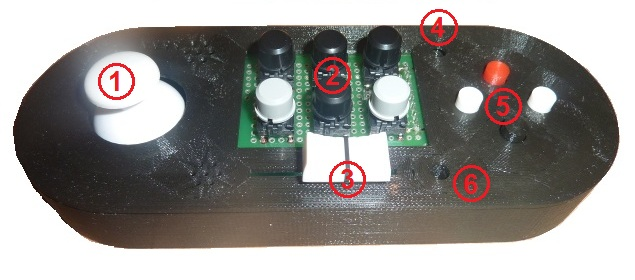
\includegraphics[width=0.8\textwidth]{controls_labeled.jpg}
\caption{Controls (Sensors) of {\Bezeichnung}}
\label{fig:controls}
\end{figure}

The listed controls of {\Bezeichnung} emulate keyboard and mouse:

\begin{table}[h]
\centering
\renewcommand{\arraystretch}{1.5}
\begin{tabular}{|p{0.05\textwidth}|p{0.25\textwidth}|p{0.60\textwidth}|}
\hline
\textbf{num.}		&	\textbf{Element}	&	\textbf{Function}\\
\hline
		1)			&	joystick			&	mouse movement\\
\hline
		2)			&	TinkerKit switches	&	mouse buttons, keyboard\\
\hline
		3)			&	slider				&	mouse scroll wheel\\
\hline
		4)			&	light sensor		&	\textit{usually disabled}\\
\hline
		5)			&	cursor pushbuttons	&	cursor key codes\\
\hline
		6)			&	three-colour LED	&	shows the selected assignment\\
\hline
\end{tabular}
\vspace{0.5cm}
\caption{Controls (Sensors) of {\Bezeichnung}}
\end{table}

\subsection*{Joystick}
The joystick usually emulates mouse movements. Depending on the
displacement of the joystick, the speed of the mouse movement is
adjusted. Pressing the joystick emulates a click on the left mouse
button.\\
On the Esplora board, the joystick is converted by two potentiometers,
whose position is read via A/D converters of the built-in 8-bit ATMEL
microcontroller \textit{ATmega32U4}. When the joystick is pressed, a
push button is actuated which is digitally read.

\subsection*{TinkerKit Switches}
On the {\Bezeichnung} there is a small additional printed circuit board
at the place where a small display would actually be installed. On this
additional board there are six pushbuttons, which are connected to the
four TinkerKit connectors. The white TinkerKit connectors are
implemented as analogue inputs, so that a sophisticated voltage divider
combination can be used to differentiate which key combination is
pressed.\\
These six buttons are assigned to additional keyboard codes or mouse
clicks.

\subsection*{Slider}
The slider control is a potentiometer connected to an A/D converter of 
the ATMEL microcontroller. It usually emulates the scrolling wheel of
the mouse.\\
Of course simply releasing the slider is not sufficient to stop the
emulated scrolling wheel! Rather, the controller must be pushed a little
bit in the opposite direction to stop the scrolling process.

\subsection*{Light Sensor}
The light sensor is connected to another A/D converter of the ATMEL
microcontroller. Some tests of the light sensor showed quickly that it
cannot be implemented as a kind of actuator. Even lightweight shadowing
will result in missinterpretations. Nevertheless the Arduino sketch
still contains some software routines to implement a control element.
However, the light sensor is disabled in most assignment modes.

\subsection*{Cursor Pushbuttons}
These four pushbuttons are digitally read by the ATMEL microcontroller.
They emulate keyboard codes to control the cursor or for moving a game
character by emulating the keys A, W, S and D. Many computer
games expect these keys.

\subsection*{Three-coloured LED}
The three-coloured LED shows the selected controller assignment (mode)
by changing its colour. See section \ref{sect:assignment}

\section{Selecting the Assignment Mode of the Actuators}
\label{sect:assignment}
Pressing all four cursor pushbuttons simultaneously starts the
setting mode of the {\Bezeichnung}. Using the UP and DOWN pushbuttons
will change the assignment of the acutators. The colour of the
three-colour LED changes according to the currently selected
assignment.\\
By pressing all four cursor pushbuttons simultaneously again, the
setting mode of the device will be quit. To prevent accidental changes
of the selected assignment mode, it is recommended to start with
pressing the cursor pushbutton LEFT or RIGHT and then pressing the
others.

\begin{table}[h]
\centering
\renewcommand{\arraystretch}{1.5}
\begin{tabular}{|p{0.05\textwidth}|p{0.15\textwidth}|p{0.70\textwidth}|}
\hline
\textbf{num.}		&	\textbf{LED colour}		&	\textbf{denomination}\\
\hline
		0)			&	\textit{``dark white''}	&	common 1\\
\hline
		1)			&	red						&	MinecraftPi\\
\hline
		2)			&	green					&	yamuplay \textit{t.b.d. (to be defined)}\\
\hline
		3)			&	yellow					&	<<undefined 3>>\\
\hline
		4)			&	blue					&	<<undefined 4>>\\
\hline
		5)			&	magenta					&	<<undefined 5>>\\
\hline
		6)			&	cyan					&	<<undefined 6>>\\
\hline
		7)			&	white					&	common 2\\
\hline
\end{tabular}
\vspace{0.5cm}
\caption{The Eight Assignment Modes for the Actuators of \Bezeichnung}
\end{table}
 
\uline{\textbf{common 1: } LED: ``dark white'' (low light emission)}\\
In this assignment mode the actuators emulate solely keyboard codes. No
mouse functions are used.

\begin{tabular}{ll}
	joystick			&	cursor keys\\
	joystick pushbutton	&	ENTER key\\
	slider				&	Pg-up, pg-dn\\
	light sensor		&	\textit{inactive}\\
	TinkerKit orange	&	SPACE key, ESC key\\
	TinkerKit white		&	modifier keys SHIFT, CTRL, ALT\\
\end{tabular}

	
\uline{\textbf{MinecraftPi: } LED: red}\\
The assignment is adapted for the game \textit{MinecraftPi} for the
\RPi.

\begin{tabular}{ll}
	joystick			&	mouse movement (to adjust the viewing angle)\\
	joystick pushbutton	&	key \texttt{E} to open the Minecraft block select menu\\
	slider				&	mouse scrolling wheel for quick block selection\\
	light sensor		&	\textit{inactive}\\
	TinkerKit orange	&	left and right mouse button\\
	TinkerKit white		&	keys ENTER, SHIFT, ESC, SPACE\\
\end{tabular}
	
	
\uline{\textbf{yamuplay: } LED: green}\\
Here it is planned to implement an assignment for controlling 
{\autor}'s media player \textit{yamuplay.py}.\\
\url{https://github.com/schlizbaeda/yamuplay}

Currently this is an undefined assignment mode!

\uline{\textbf{<<undefined 3>>: } LED: yellow}\\
This is an undefined assignment mode!

\uline{\textbf{<<undefined 4>>: } LED: blue}\\
This is an undefined assignment mode!

\uline{\textbf{<<undefined 5>>: } LED: magenta}\\
This is an undefined assignment mode!

\uline{\textbf{<<undefined 6>>: } LED: cyan}\\
This is an undefined assignment mode!

\uline{\textbf{common 2: } LED: white}\\
This mode emulates keyboard and mouse actions.

\begin{tabular}{ll}
	joystick			&	mouse movement\\
	joystick pushbutton	&	left mouse button\\
	slider				&	mouse scrolling wheel\\
	light sensor		&	\textit{inactive}\\
	TinkerKit orange	&	left and right mouse button\\
	TinkerKit white		&	modifier keys SHIFT, CTRL, ALT\\
\end{tabular}
